\documentclass[11pt]{article}
\usepackage{graphicx}
\usepackage{amsthm}
\usepackage{amsmath}
\usepackage{amssymb}
\usepackage[shortlabels]{enumitem}
\usepackage[margin=1in]{geometry}
\usepackage{pgfplots}

\newcommand{\N}{\mathbb{N}}

\newenvironment{solution}
  {\renewcommand\qedsymbol{$\blacksquare$}\begin{proof}[Solution]}
  {\end{proof}}

\setlength\parindent{0pt}

\newtheorem*{observation}{Observation}
\newtheorem*{theorem}{Theorem}
\newtheorem*{claim}{Claim}
\newtheorem*{corollary}{Corollary}

\theoremstyle{definition}
\newtheorem*{definition}{Definition}

\begin{document}

	\hrule
	\begin{center}
        \textbf{MATH66: Stochastic and Numerical Methods}\hfill \textbf{Fall 2023}\newline

		{\Large Homework 1}

		David Yang
	\end{center}

\hrule

\vspace{1em}

\textit{Problems from Numerical Analysis (Sauer), Chapter 1.} \\

\underline{Example 1.15, page 61} \\

\textbf{Apply Newton's Method to $f(x) = 4x^4 - 6x^2 -11/4$ with starting guess $x_0 = \frac{1}{2}.$} \\

\begin{solution} The sequence of numbers produced by Newton's method for starting guess $x_0 = \frac{1}{2}$ alternates between $\frac{1}{2}$ and $-\frac{1}{2}$:
\[ x_0 = \frac{1}{2}, \, x_1 = -\frac{1}{2}, \, x_2 = \frac{1}{2}, \dots \]

Since neither $\pm \frac{1}{2}$ is a root of $f(x)$, the sequence produced by Newton's method fails to converge to a root. \end{solution}

\vspace{1.5cm}

\underline{Section 1.4 (Newton's Method), Problem 6} \\

\textbf{Sketch a function f and initial guess for which Newton's Method diverges.} 

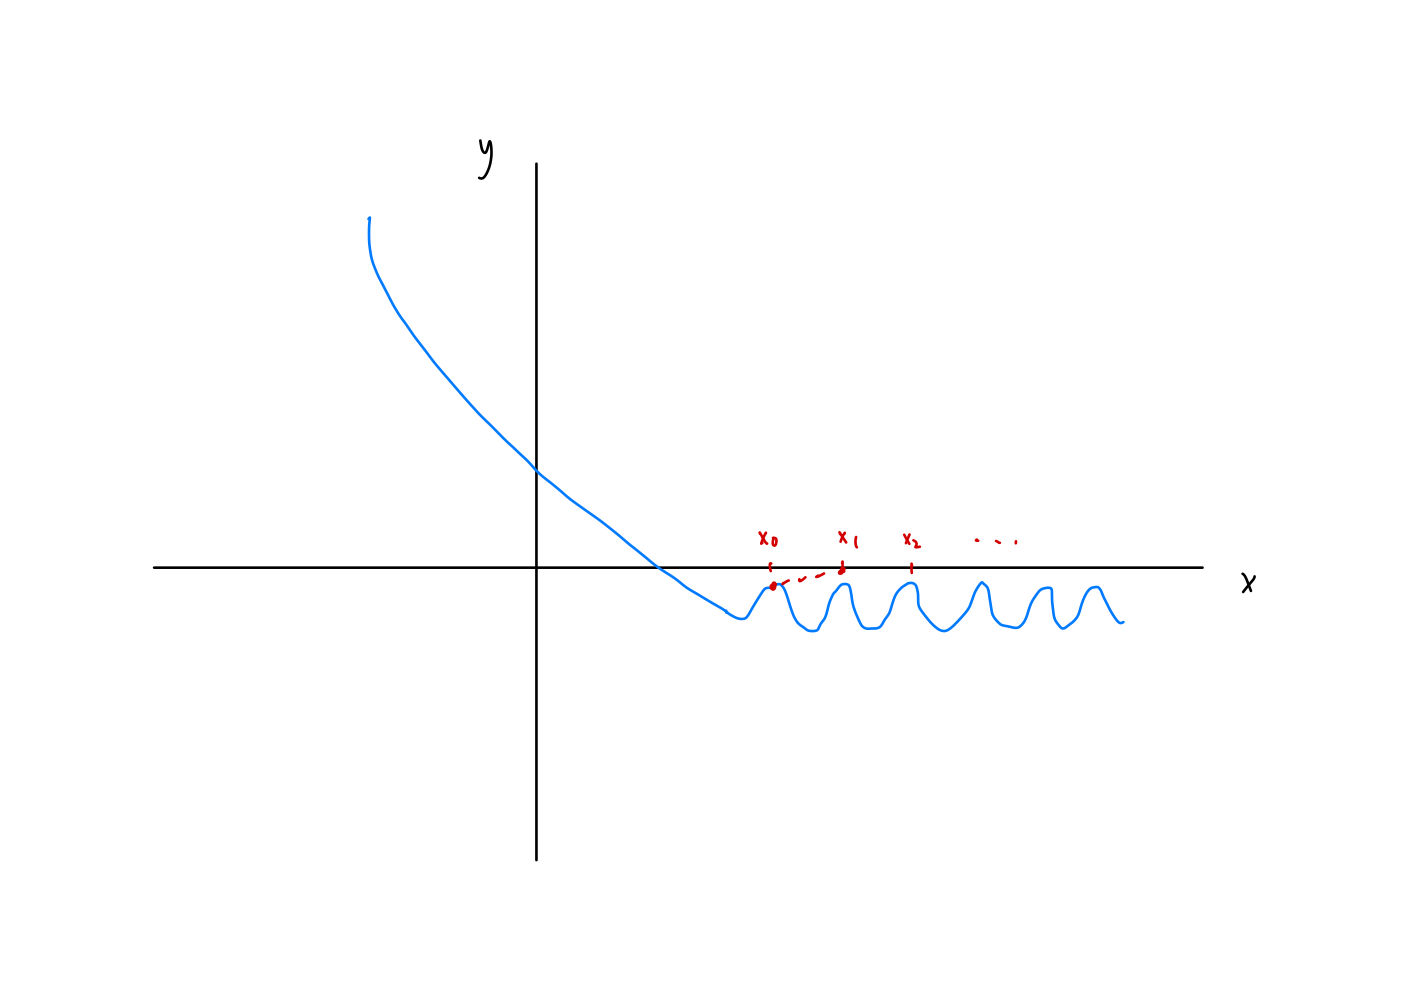
\includegraphics[scale = 0.25]{M66_1.4.6.jpeg}

\begin{solution}
    Newton's Method would diverge with the marked initial guess; the further iterations continue along the positive $x$ axis and move away from the root.
\end{solution}

\newpage

\underline{Section 1.4 (Newton's Method), Problem 8} \\


\textbf{Prove that Newton's Method applied to $f(x) = ax + b$ converges in one step.} 

\begin{solution}
Let $x_0$ be the initial guess for Newton's method, where $x_0 \neq -\frac{b}{a}$ (assumed to not be the root). We know that $f'(x_0) = a$. \\

Newton's method after one iteration says that 
\[ x_1 = x_0 - \frac{f(x_0)}{f'(x_0)} = x_0 - \frac{ax_0 + b}{a} = -\frac{b}{a}. \]

Note that $f(x_1) = 0$; thus, Newton's method applied to $f(x) = ax+b$ converges in one step.
\end{solution}

\vspace{1.5cm}

\underline{Section 1.5 (Root-Finding without Derivatives), Problem 1(c)} \\

\textbf{Apply two steps of the Secant Method to $e^x + \sin x = 4$ with initial guesses $x_0 = 1, x_1 = 2$.} 

\begin{solution}

First, we rearrange the equation to reform it as a root-finding problem: $f(x) = e^x + \sin x - 4.$ \\

After one step of the Secant Method, we get 
\[ x_2 = x_1 - \frac{f(x_1)(x_1 - x_0)}{f(x_1) - f(x_0)} = 2 - \frac{f(2)(2-1)}{f(2) - f(1)}. \]

Plugging in $f(2) = e^2 + \sin(2) - 4 \approx 4.298$ and $f(1) = e^1 + \sin(1) - 4 \approx -0.44$, we get that
\[ x_2 \approx 2 - \frac{4.298(2-1)}{4.298 - (-0.44)} \approx 1.093. \]

The second step of the Secant Method gives the following:
\[ x_3 = x_2 - \frac{f(x_2)(x_2 - x_1)}{f(x_2) - f(x_1)} \approx 1.093 - \frac{f(1.093)(1.093 - 2)}{f(1.093) - f(2)}. \]

Plugging in the approximations $f(1.093) \approx e^{1.093} + \sin(1.093) - 4 \approx -0.129$ and $f(2) \approx 4.298$, we get that
\[ x_3 \approx 1.093 - \frac{-0.129(0.129 - 2)}{-0.129 - 4.298} \approx \boxed{1.1193}. \]

As we can see, after two steps, the result from Newton's method approaches the true root, $r \approx 1.13.$
\end{solution}
\end{document}